\documentclass[12pt]{article}
\usepackage[utf8]{inputenc}
\usepackage{graphicx}
\usepackage{listings}
\usepackage{amsmath}
\graphicspath{ {./images/} }
\usepackage{amssymb}
\usepackage[htt]{hyphenat}

\usepackage{hyperref}
\hypersetup{
    colorlinks=true,
    linkcolor=blue,
    filecolor=magenta,      
    urlcolor=cyan,
}

\usepackage{xcolor}

\definecolor{codegreen}{rgb}{0,0.6,0}
\definecolor{codegray}{rgb}{0.5,0.5,0.5}
\definecolor{codepurple}{rgb}{0.58,0,0.82}
\definecolor{backcolour}{rgb}{0.95,0.95,0.92}
\definecolor{codeorange}{rgb}{1,0.64,0}

\lstdefinestyle{mystyle}{
    backgroundcolor=\color{backcolour},   
    commentstyle=\color{codegreen},
    keywordstyle=\color{magenta},
    numberstyle=\tiny\color{codeorange},
    stringstyle=\color{codepurple},
    basicstyle=\ttfamily\footnotesize,
    breakatwhitespace=false,         
    breaklines=true,                 
    captionpos=b,                    
    keepspaces=true,                 
    numbers=left,                    
    numbersep=5pt,                  
    showspaces=false,                
    showstringspaces=false,
    showtabs=false,                  
    tabsize=2
}

\lstset{style=mystyle, breaklines=true, postbreak=\mbox{\textcolor{red}{$\hookrightarrow$}\space}}

\title{\vspace{-1cm}Laplace Equation\\
\large Assignment 5\\
\large EE2703 - Applied Programming Lab}
\author{Abhigyan Chattopadhyay \\
EE19B146}
\date{30th March 2021}
\usepackage[margin=0.75in]{geometry}

\begin{document}

\maketitle
\tableofcontents
\pagebreak
\section{The Problem at Hand}
We are trying to solve the Laplace equation to find out which region of a resistor placed on a 1cm$\times$1cm Copper plate gets the hottest, by finding the temperature distribution over the entire Copper plate.

We will plot the temperature gradients and visualise the distribution to find which locations are the hottest.

We will also try to understand the effectiveness and efficiency of solving the Laplace equation using this method.
\begin{center}
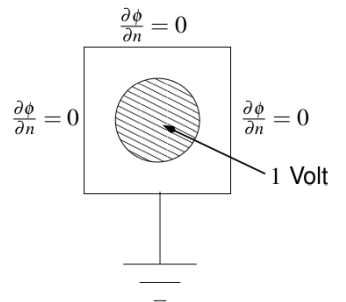
\includegraphics{images/fig0.png}
\end{center}

Now, we know that:
\begin{itemize}
    \item $\vec{j} = \sigma \vec{E}$ (Ohm's Law)

    \item $\vec{E} = -\nabla \phi$ (Electric field is gradient of potential)

    \item $\nabla \cdot \vec{j} = \frac{\partial \rho}{\partial t}$ (Continuity equation)
\end{itemize}

On combining these, we get:

\begin{itemize}
    \item $\nabla (-\sigma \nabla \phi) = \frac{\partial \rho}{\partial t}$
\end{itemize}

And assuming constant conductivity, we get:

\begin{itemize}
    \item $\nabla^2\phi = \frac{1}{\sigma} \frac{\partial \rho}{\partial t}$
\end{itemize}

And for DC currents, $\frac{\partial \rho}{\partial t} = 0$, and hence:

$$\nabla ^2 \phi = 0$$

And in 2 Dimensions:

$$\frac{\partial^2 \phi}{\partial x^2} + \frac{\partial^2 \phi}{\partial y^2} = 0$$

This is nothing but the Laplace equation, which we will now solve numerically.
\pagebreak
\section{Numerical Solution to the Laplace Equation}

\begin{center}
\boxed{\frac{\partial^2 \phi}{\partial x^2} + \frac{\partial^2 \phi}{\partial y^2} = 0}
\end{center}

We will discretize the x and y space in order to solve our equation numerically. And in a discrete space, we can say:

$$\frac{\partial^2 \phi}{\partial x^2} = \frac{\phi(x_{i+1},y_{j})+\phi(x_{i-1},y_{j}) - 2\phi(x_i,y_j)}{(\Delta x)^2}$$

$$\frac{\partial^2 \phi}{\partial y^2} = \frac{\phi(x_{i},y_{j+1})+\phi(x_{i},y_{j-1}) - 2\phi(x_i,y_j)}{(\Delta y)^2}$$

And, on replacing this into the Laplace Equation, we get:

\begin{center}
\boxed{\phi(x_{i},y_{j}) = \frac{\phi(x_{i+1},y_{j}) + \phi(x_{i-1},y_{j}) + \phi(x_{i},y_{j+1}) + \phi(x_{i},y_{j-1})}{4}}
\end{center}

(Note that this assumes that $\Delta x = \Delta y$)

Now, we need to substitute the right boundary conditions to get the overall temperature distribution over our region of interest, in this case, the copper plate.

Here, our boundary conditions are given as:

\begin{itemize}
    \item $\phi = 1V$ at the place of contact of the electrode with the copper plate.
    \item $\phi = 0V$ at the bottom edge which is grounded
\end{itemize}


\section{Potential Distribution}

\subsection{Parameters}

We have 4 main parameters:

\begin{enumerate}
    \item $N_x$ and $N_y$: These are the horizontal and vertical number of divisions respectively, which are used to discretize the space. We take both their values as 25 by default.
    \item $R$: Radius of the electrode in units of $\frac{1cm}{Nx}$ or $\frac{1cm}{Ny}$. We take it as 8 units by default here.
    \item $N_{iter}$: The number of iterations while solving the Laplace Equation. We take it as 1500 by default here.
\end{enumerate}

These can be supplied as Command Line Arguments, but if not specified, then their default values are taken.

\subsection{Initial State}
\begin{center}
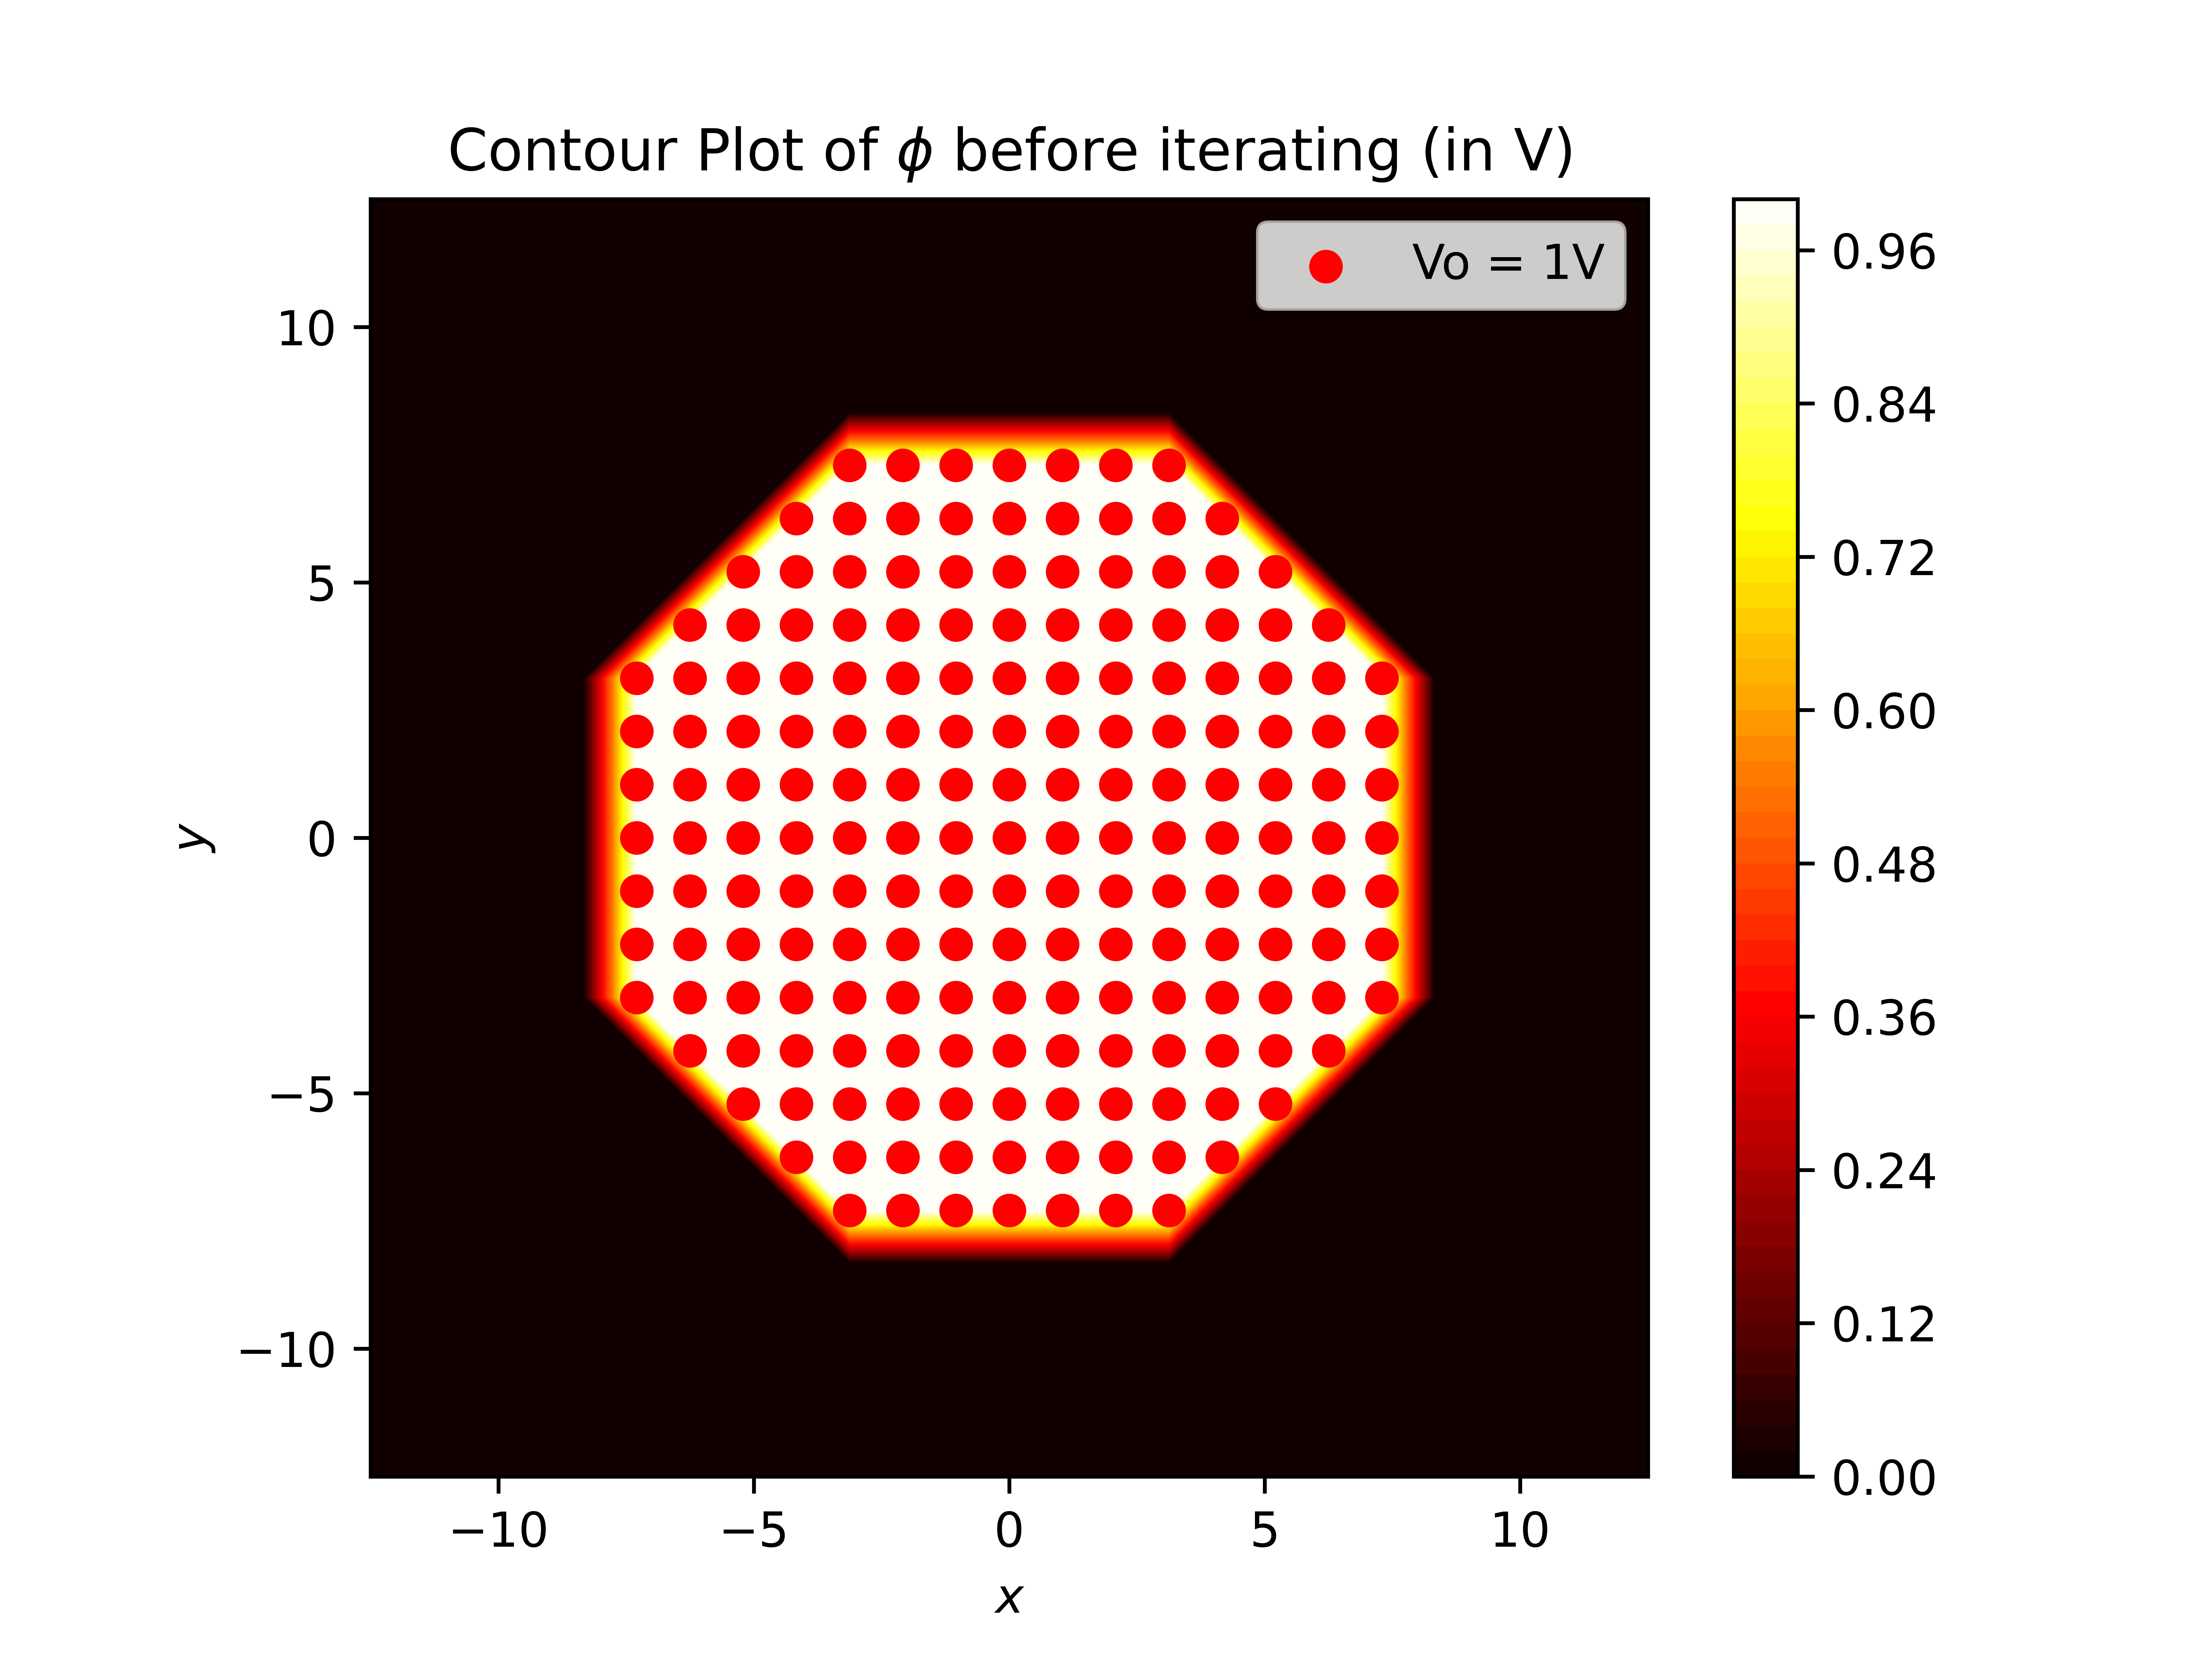
\includegraphics{images/fig1.png}
\end{center}
\tiny{(Colormap used: cm.hot)}

\normalsize
As is clearly visible, the potential is 0 in all areas except in the central circular region where the electrode is in contact with the plate.

(Note that it appears octagonal due to discretization)

Now, we will solve the Laplace equation and store the error with respect to itself over time.
\pagebreak
\subsection{Final State}

As a 3D surface plot (using cm.jet):
\begin{center}
    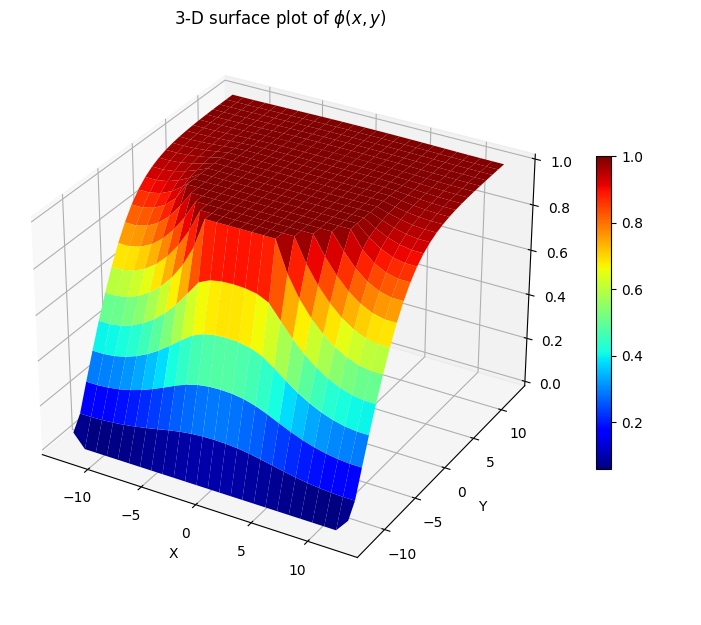
\includegraphics{images/fig4_2.png}
\end{center}
\pagebreak
As a contour plot (using cm.hot)
\begin{center}
    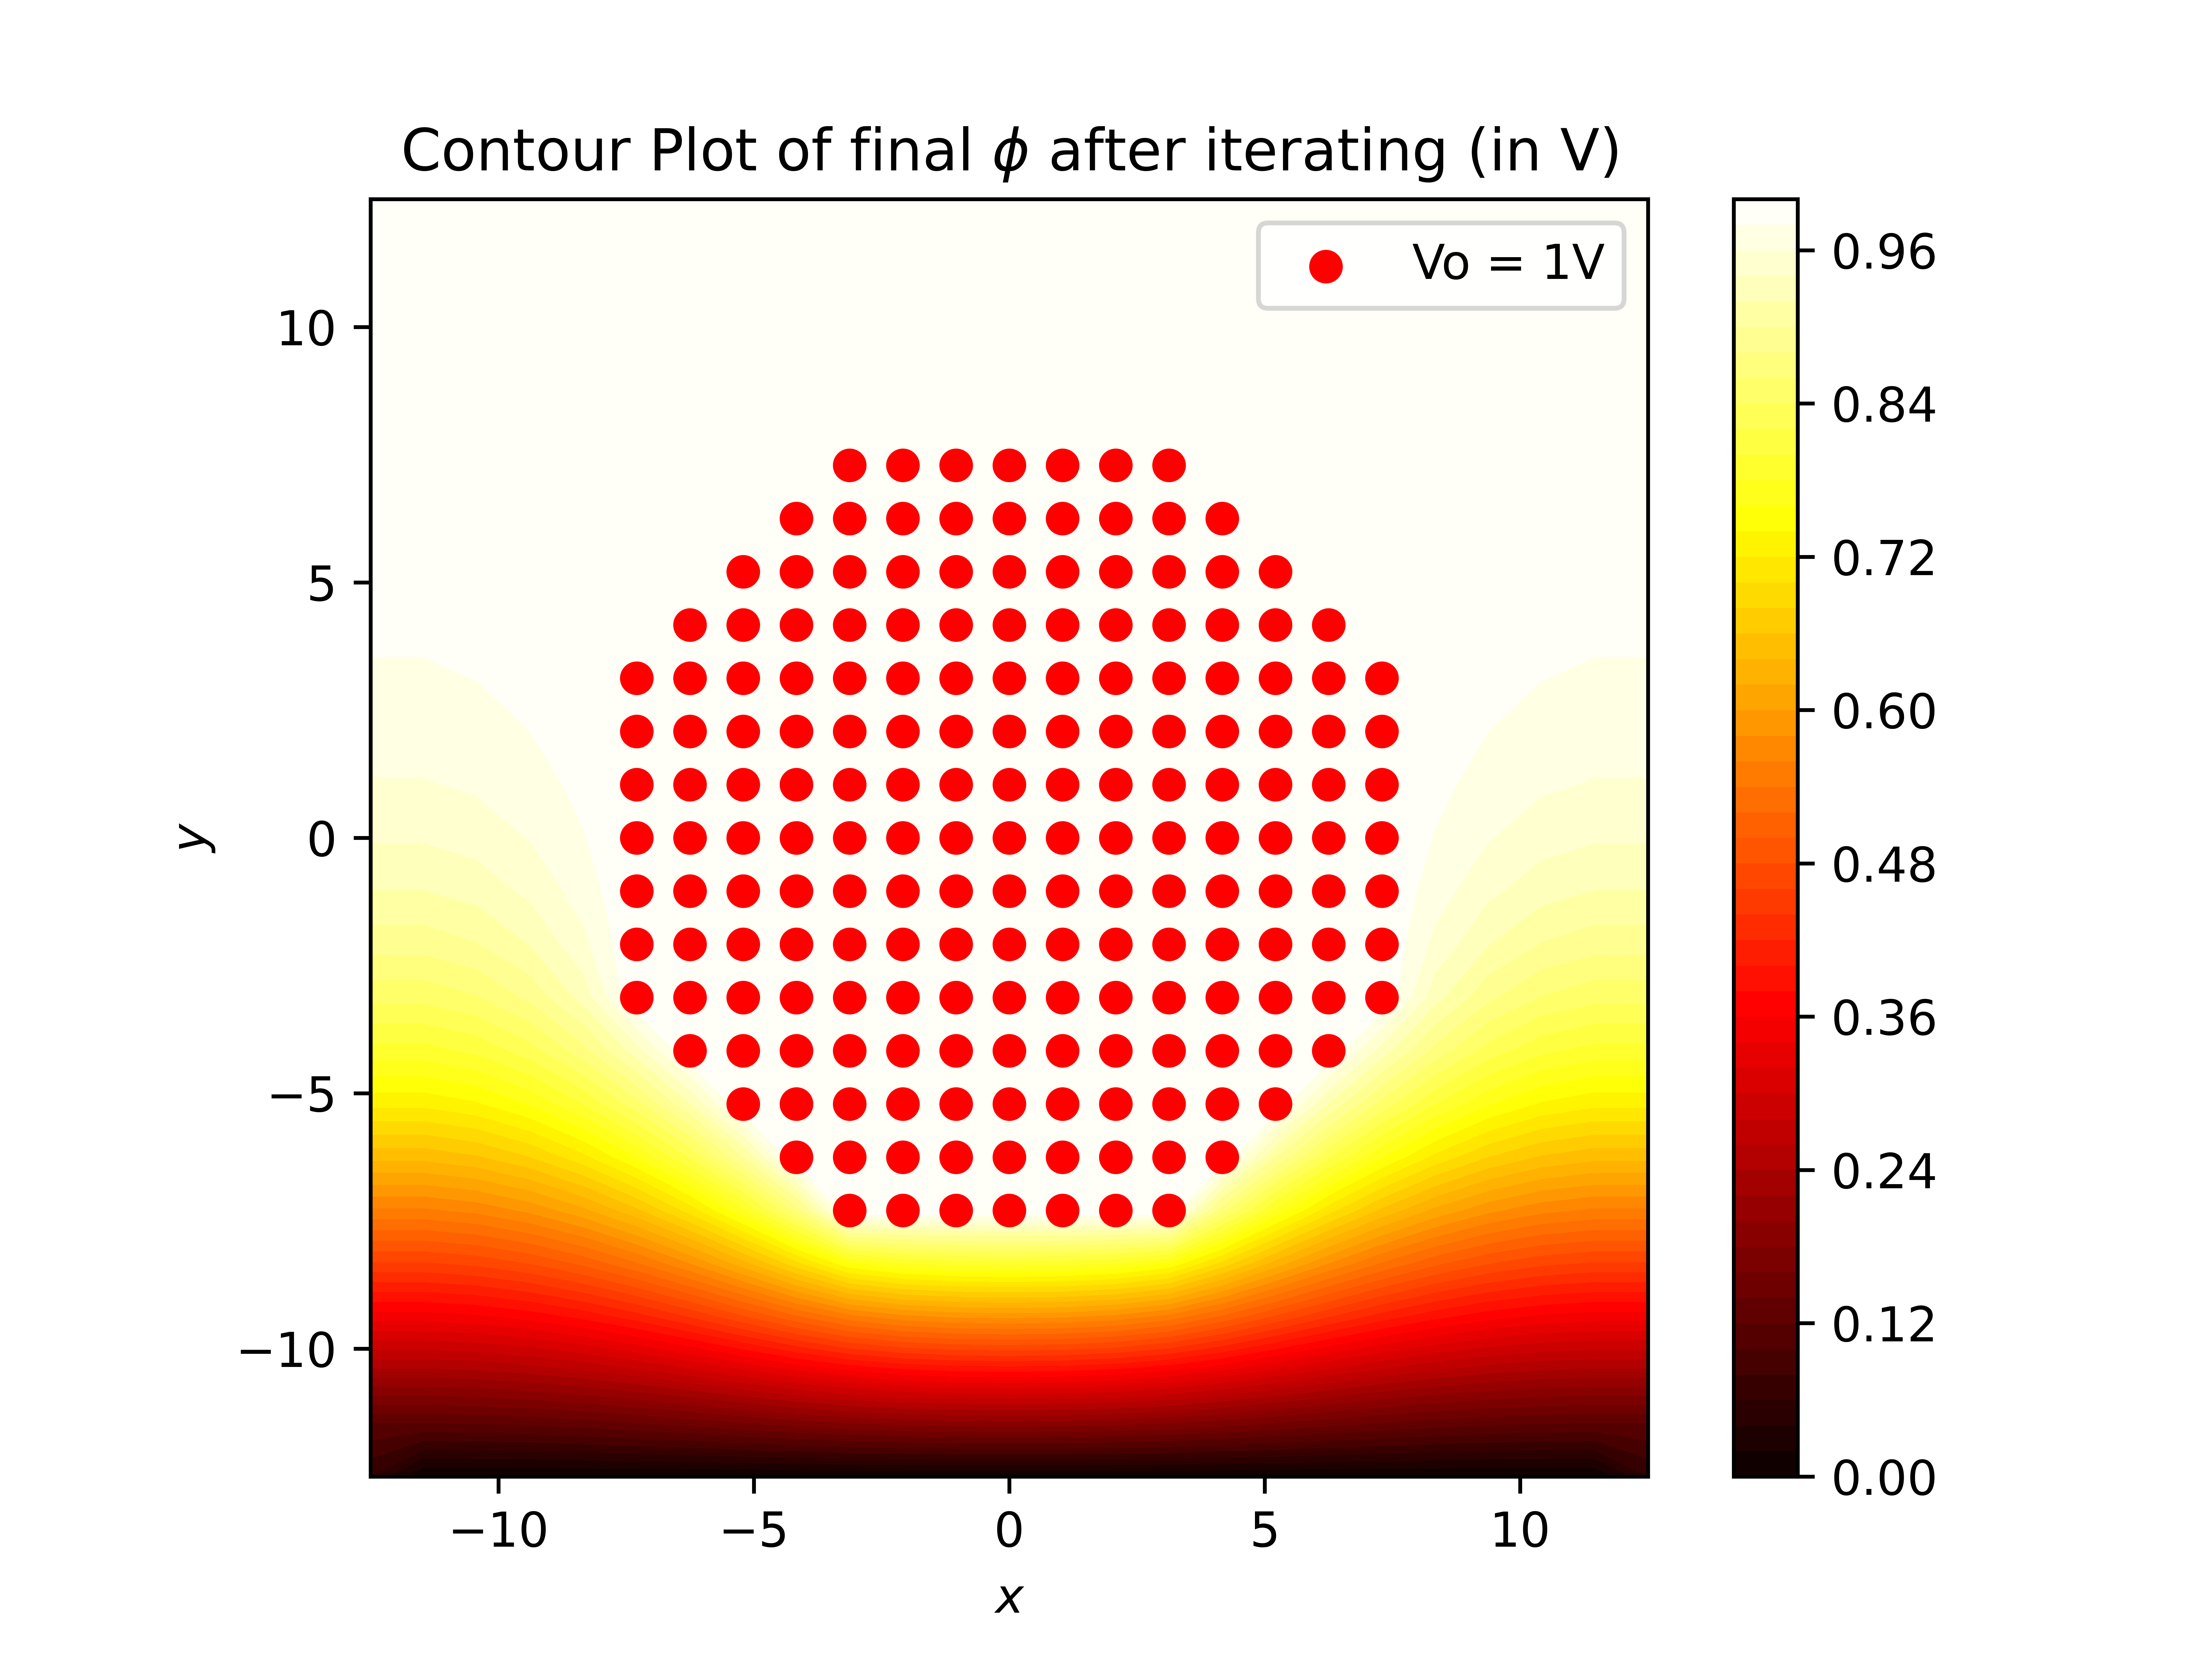
\includegraphics{images/fig5.png}
\end{center}
\pagebreak
\subsection{Error Analysis}
Now, we will plot the error values as calculated and then try to fit a line to it using \texttt{lstsq}.

We will first fit a line through all the error data points, and then through the errors after the 500th iteration only.

We will only be using every 50th sample to do this, as using every sample makes the task extremely computationally intensive.

This is plotted on a semi-log scale, and the plot obtained is shown below:
\begin{center}
    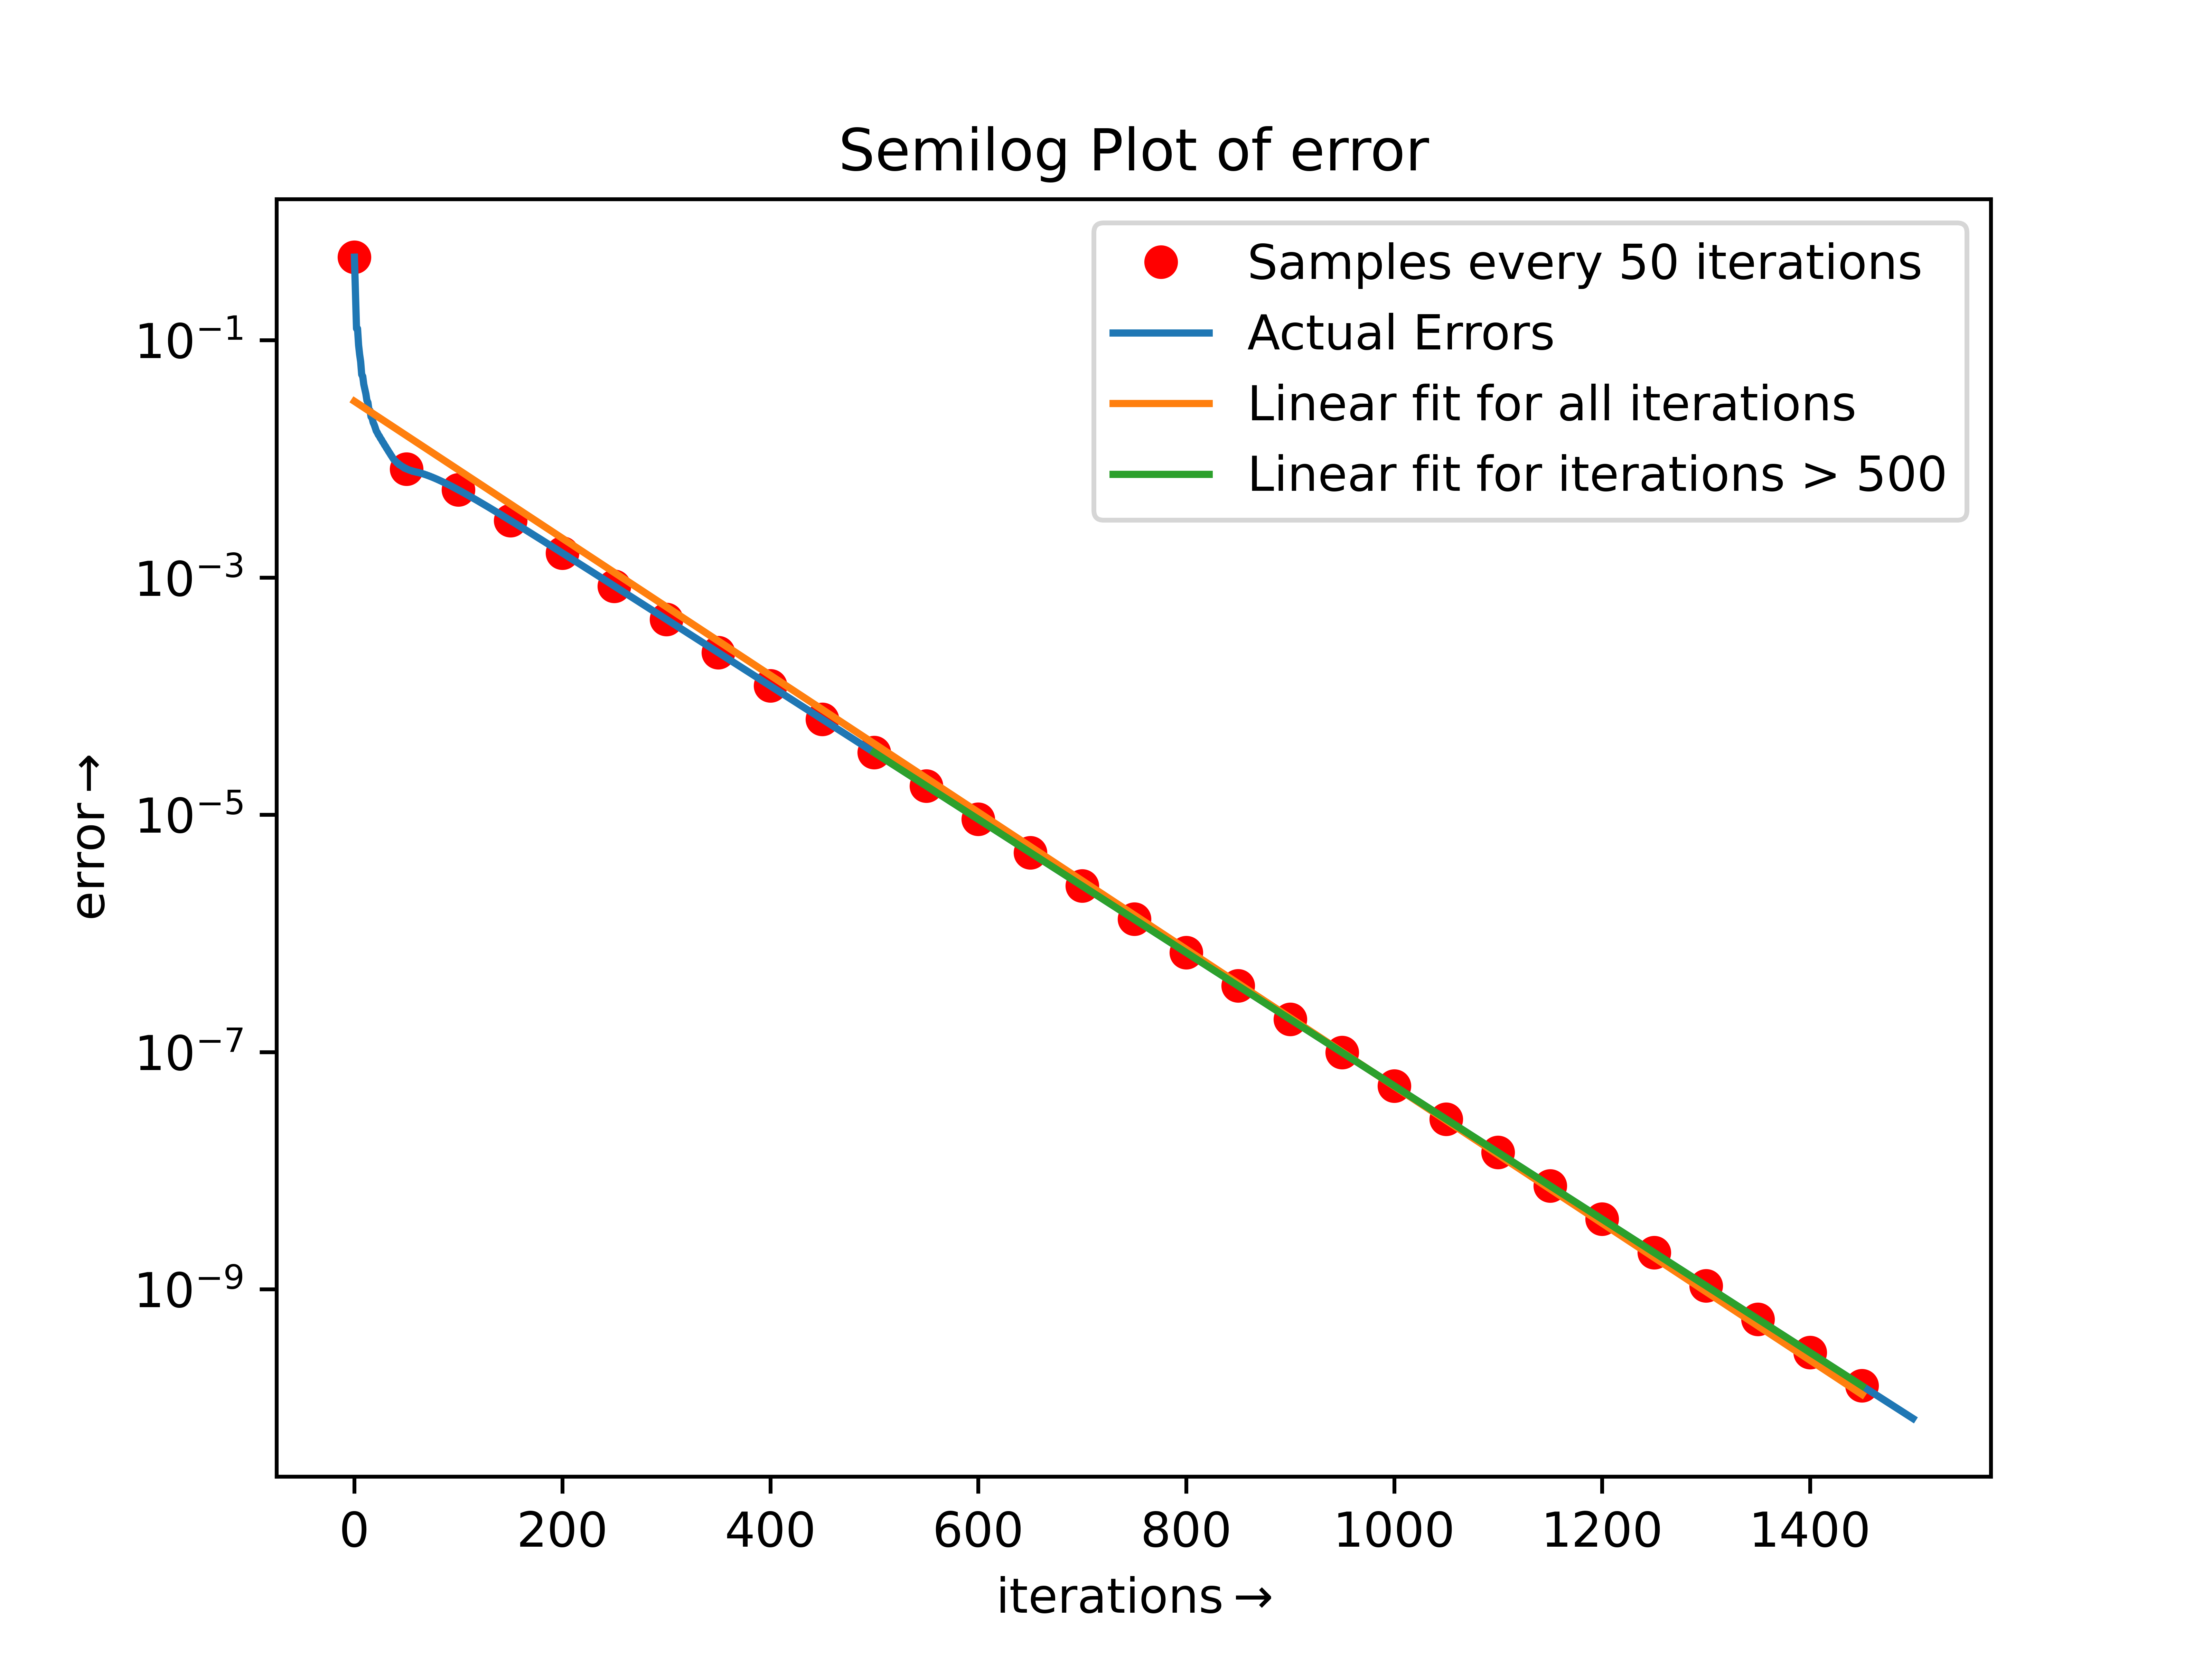
\includegraphics[scale=0.8]{images/fig2.png}
\end{center}
\pagebreak
Now we plot the error on a log-log scale and we get:
\begin{center}
    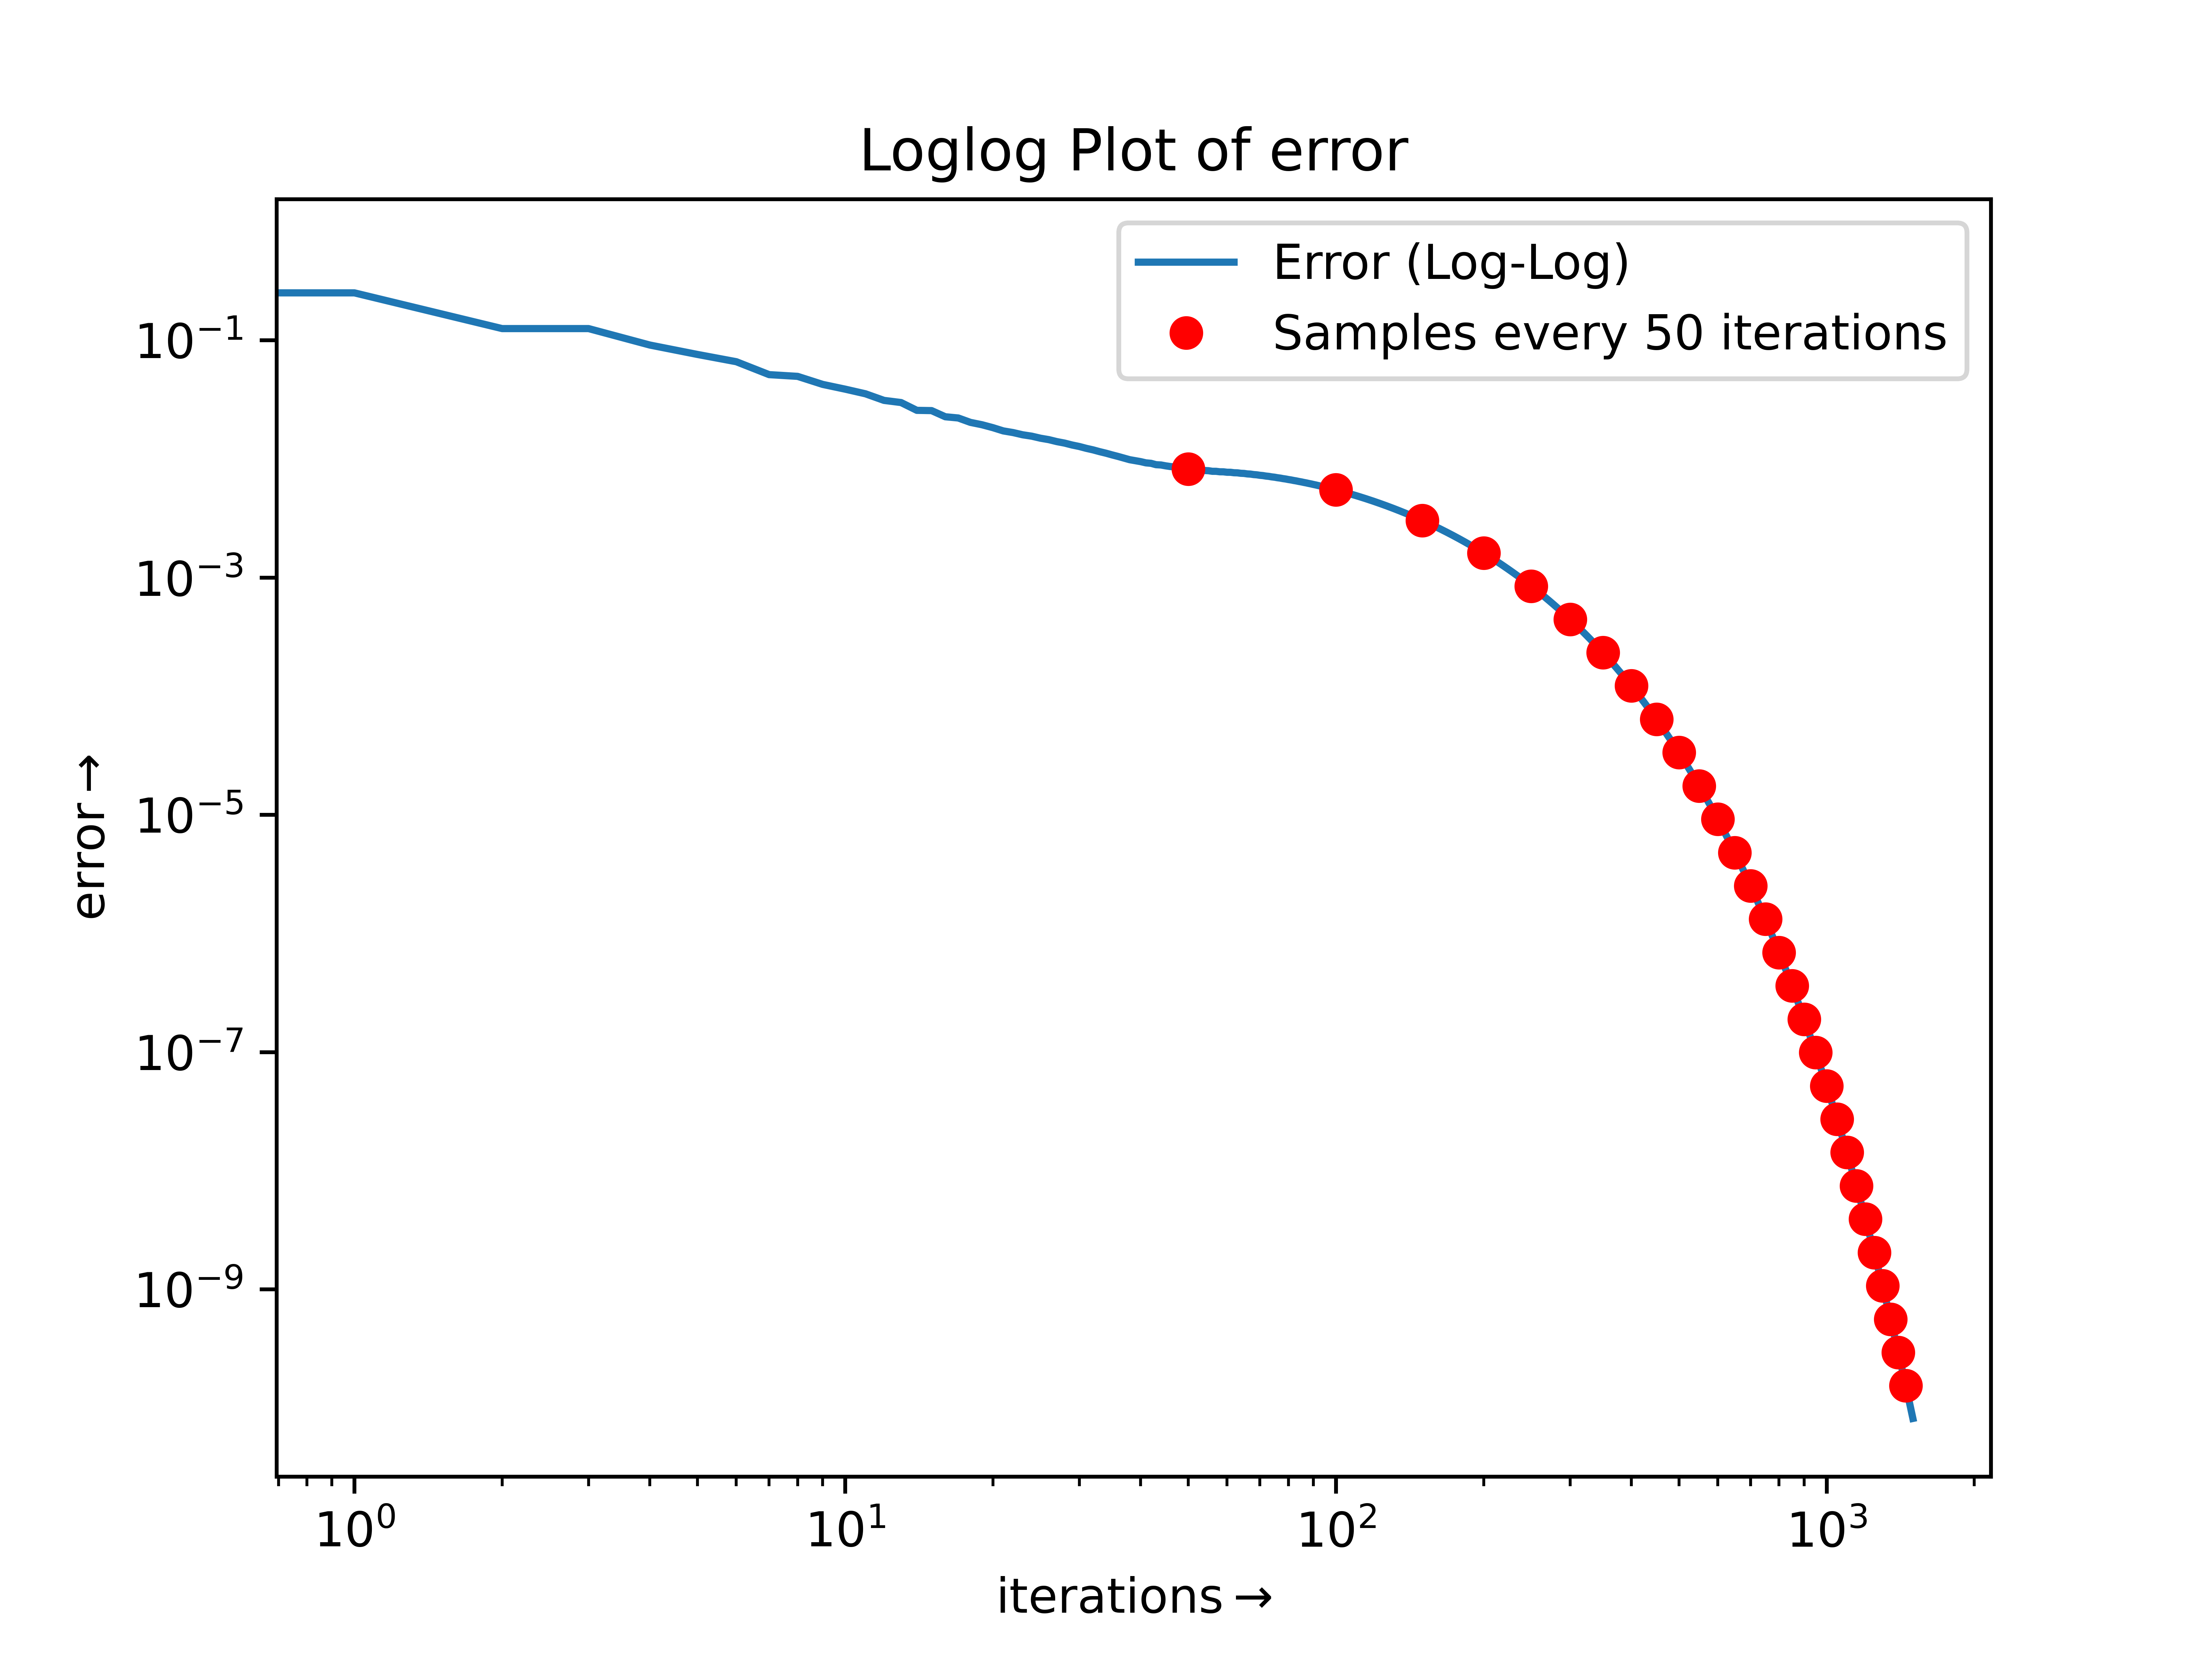
\includegraphics[scale=0.8]{images/fig3.png}
\end{center}

This shows us that the error remains approximately linear until 50 iterations, but becomes exponential after that.

\subsection{Stopping Condition}
Solving the Laplace equation numerically requires a pre-determined number of iterations, which acts as a built-in stopping condition for us as of now.

However, we need to be able to determine this by ourselves, and can do so using the parameters that we have estimated using the \texttt{lstsq} earlier.

Our error can be approximated as $Ae^{Bk}$, and when we apply log on both sides and fit the error to the resulting linear equation $\log{A} + B k$, we get:
$A = -3.83851276$ and $B = -0.01293527 $.

With these values, using the concept given in the assignment, our half-life for error turns out to be $\frac{1}{B} = 77.308$, and this means that it will take a really large number of iterations to converge to zero.
\pagebreak
\section{Current Density}

We saw earlier that $\vec{J} = -\sigma \nabla \phi$. If we assume $\sigma=1$, on simplifying, we get:
$$J_x = -\frac{\partial \phi}{\partial x}$$
$$J_y = -\frac{\partial \phi}{\partial y}$$

And upon discretizing, we get:

$$J_{x,ij} = \frac{1}{2}(\phi(x_{i},y_{j-1})-\phi(x_{i},y_{j+1}))$$

$$J_{y,ij} = \frac{1}{2}(\phi(x_{i},y_{j-1})-\phi(x_{i},y_{j+1}))$$

This gives us the vector $\vec{J}$, which we now plot using a quiver plot as follows:
\begin{center}
    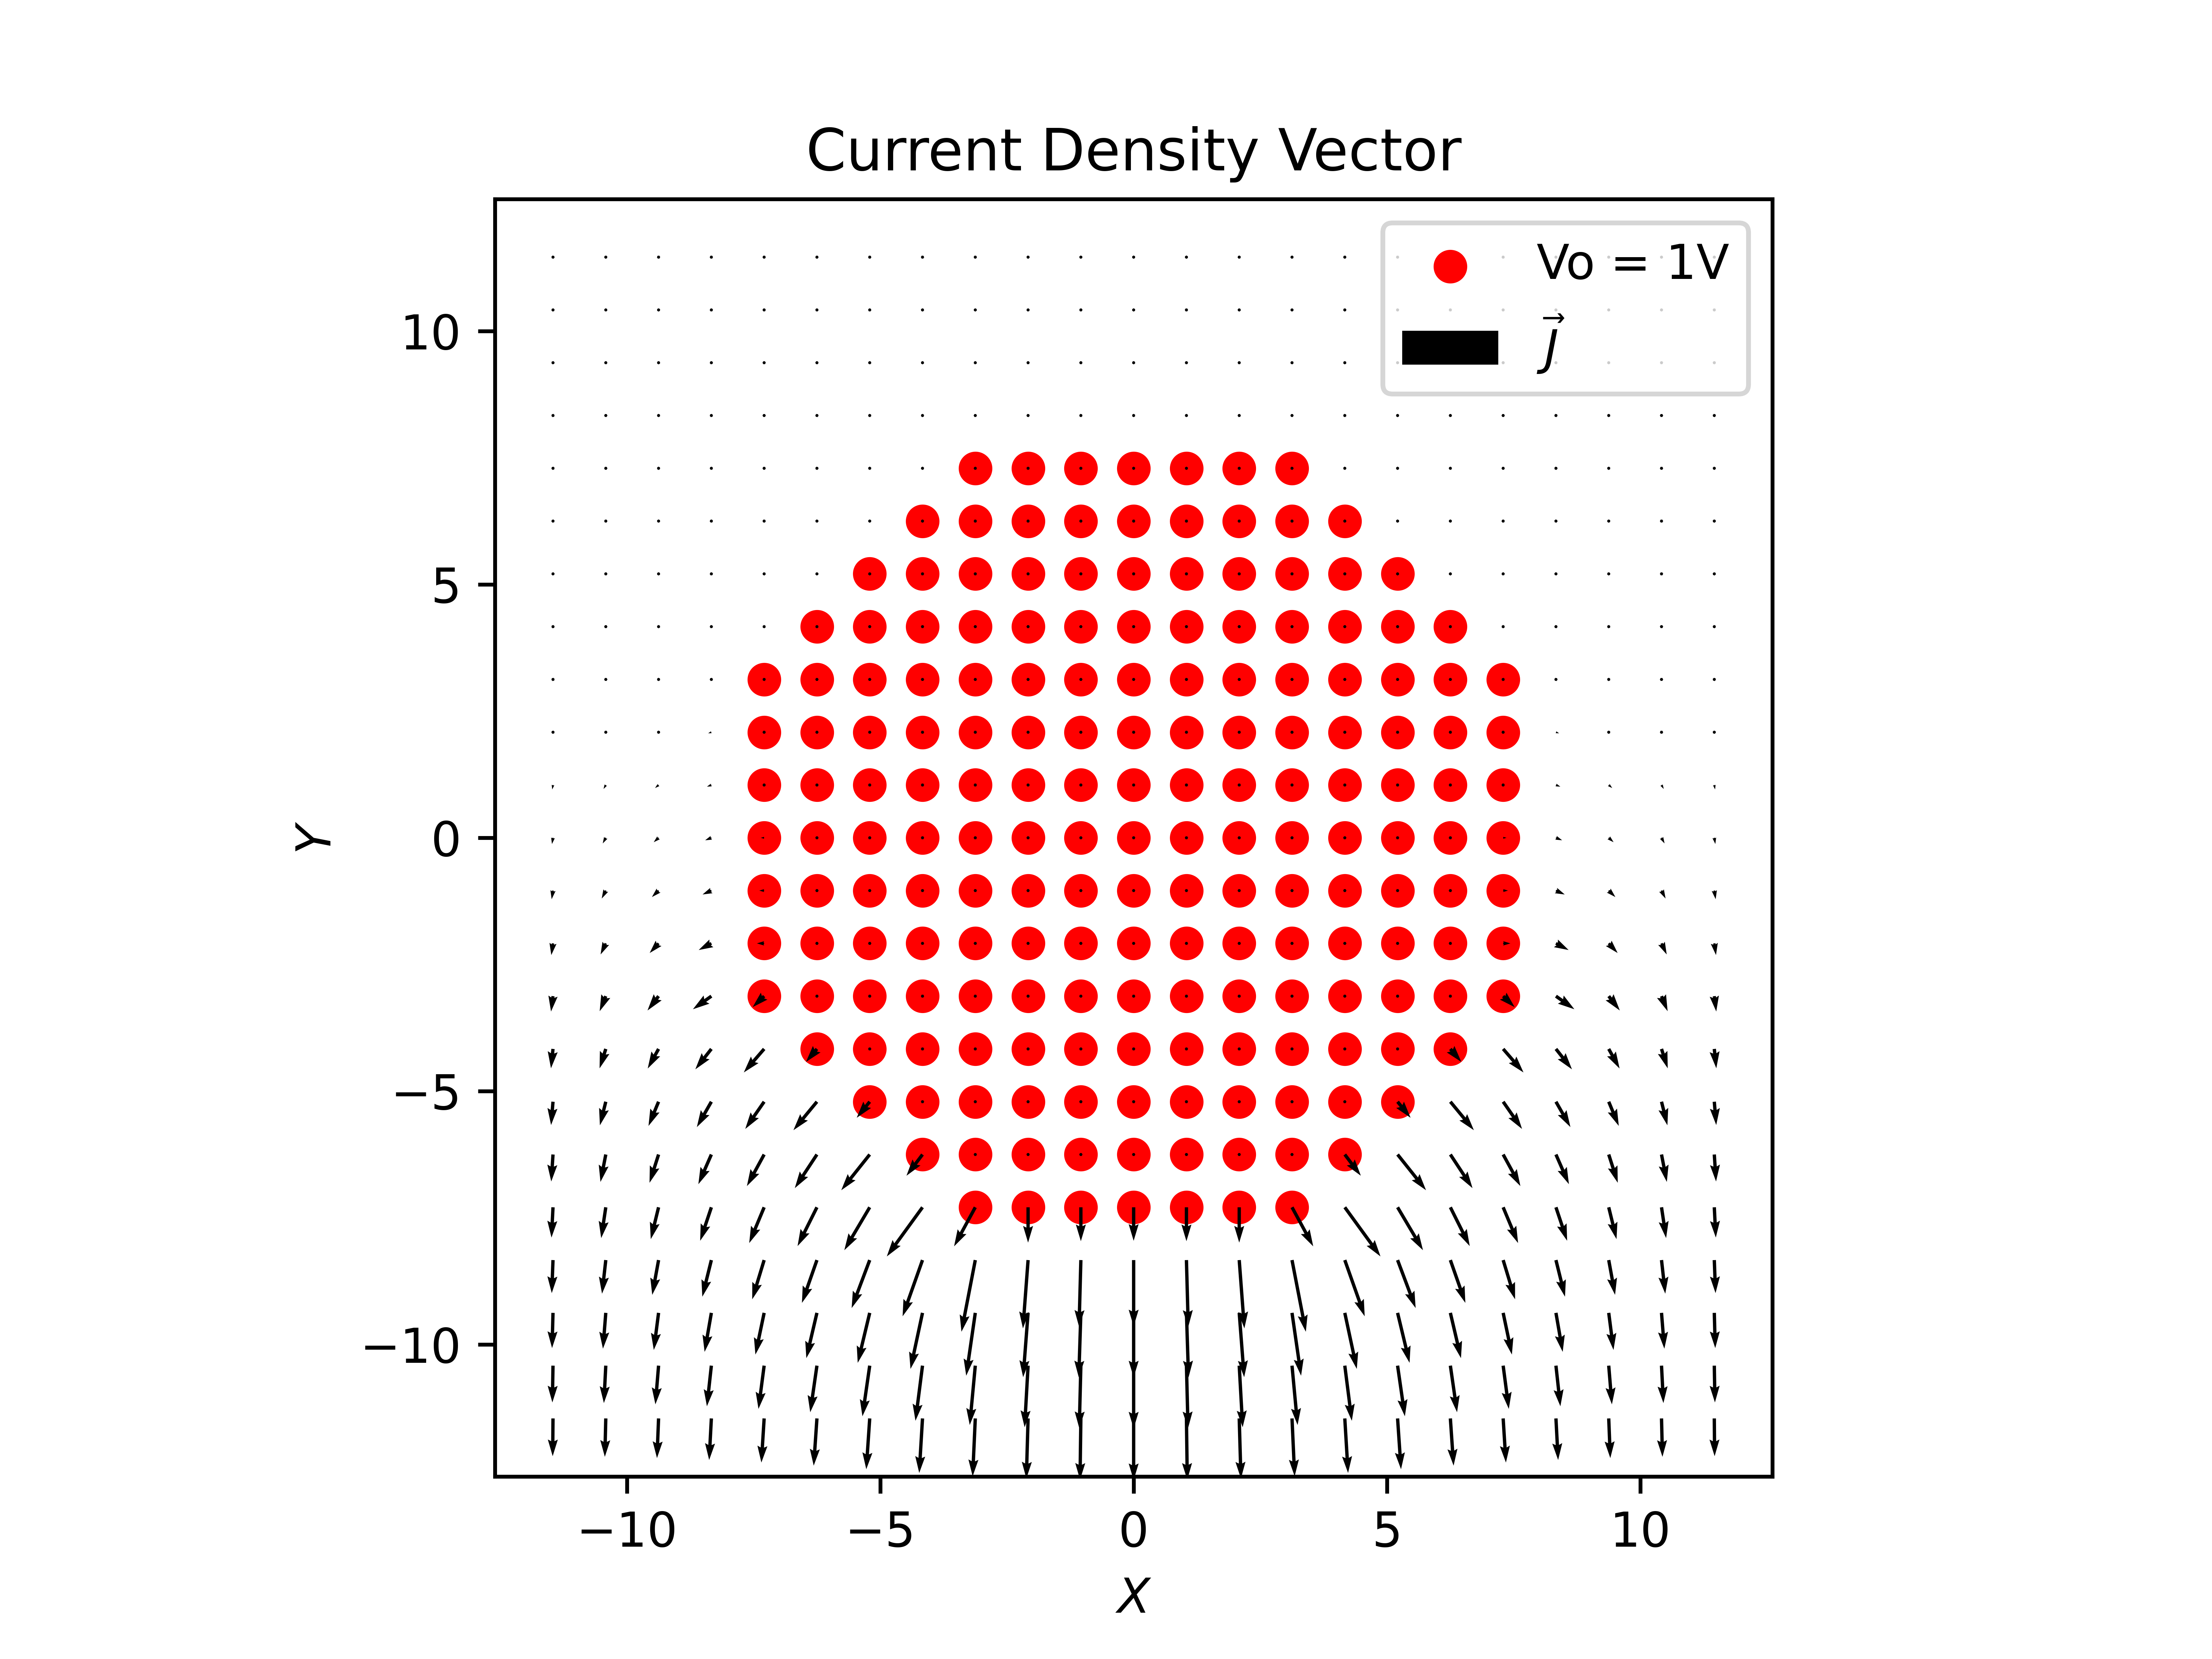
\includegraphics{images/fig6.png}
\end{center}
It is clear that the current is mostly confined to the bottom half of the plate. 
This even makes sense intuitively that the current would flow straight from the electrode into the grounded bottom edge and not go in any other direction.
\pagebreak
\section{Temperature Distribution}
Now, we will solve the Poisson's Equation for the temperature distribution over the plate, and plot it.

Using the heat equation:
$$-\nabla \cdot (\kappa \nabla T) = \frac{1}{\sigma} |\vec{J}|^2$$

After discretizing and simplifying in a similar way as we simplified the Laplace equation earlier, we have:

$$T_{i,j} = \frac{T_{i+1,j}+T_{i-1,j}+T_{i,j+1}+T_{1,j-1}}{4} + \frac{|\vec{J}|^2}{4\sigma \kappa}$$

Now we will set $\kappa \sigma = 1$, and use the following conditions:

\begin{itemize}
    \item The entire plate starts out at room temperature (300K)
    \item Electrode contact area is always at 300K
    \item Bottom edge is always at 300K
    \item $\frac{\partial T}{\partial n} = 0$ at the other three edges
\end{itemize}

This gives us the following temperature distribution:

\begin{center}
    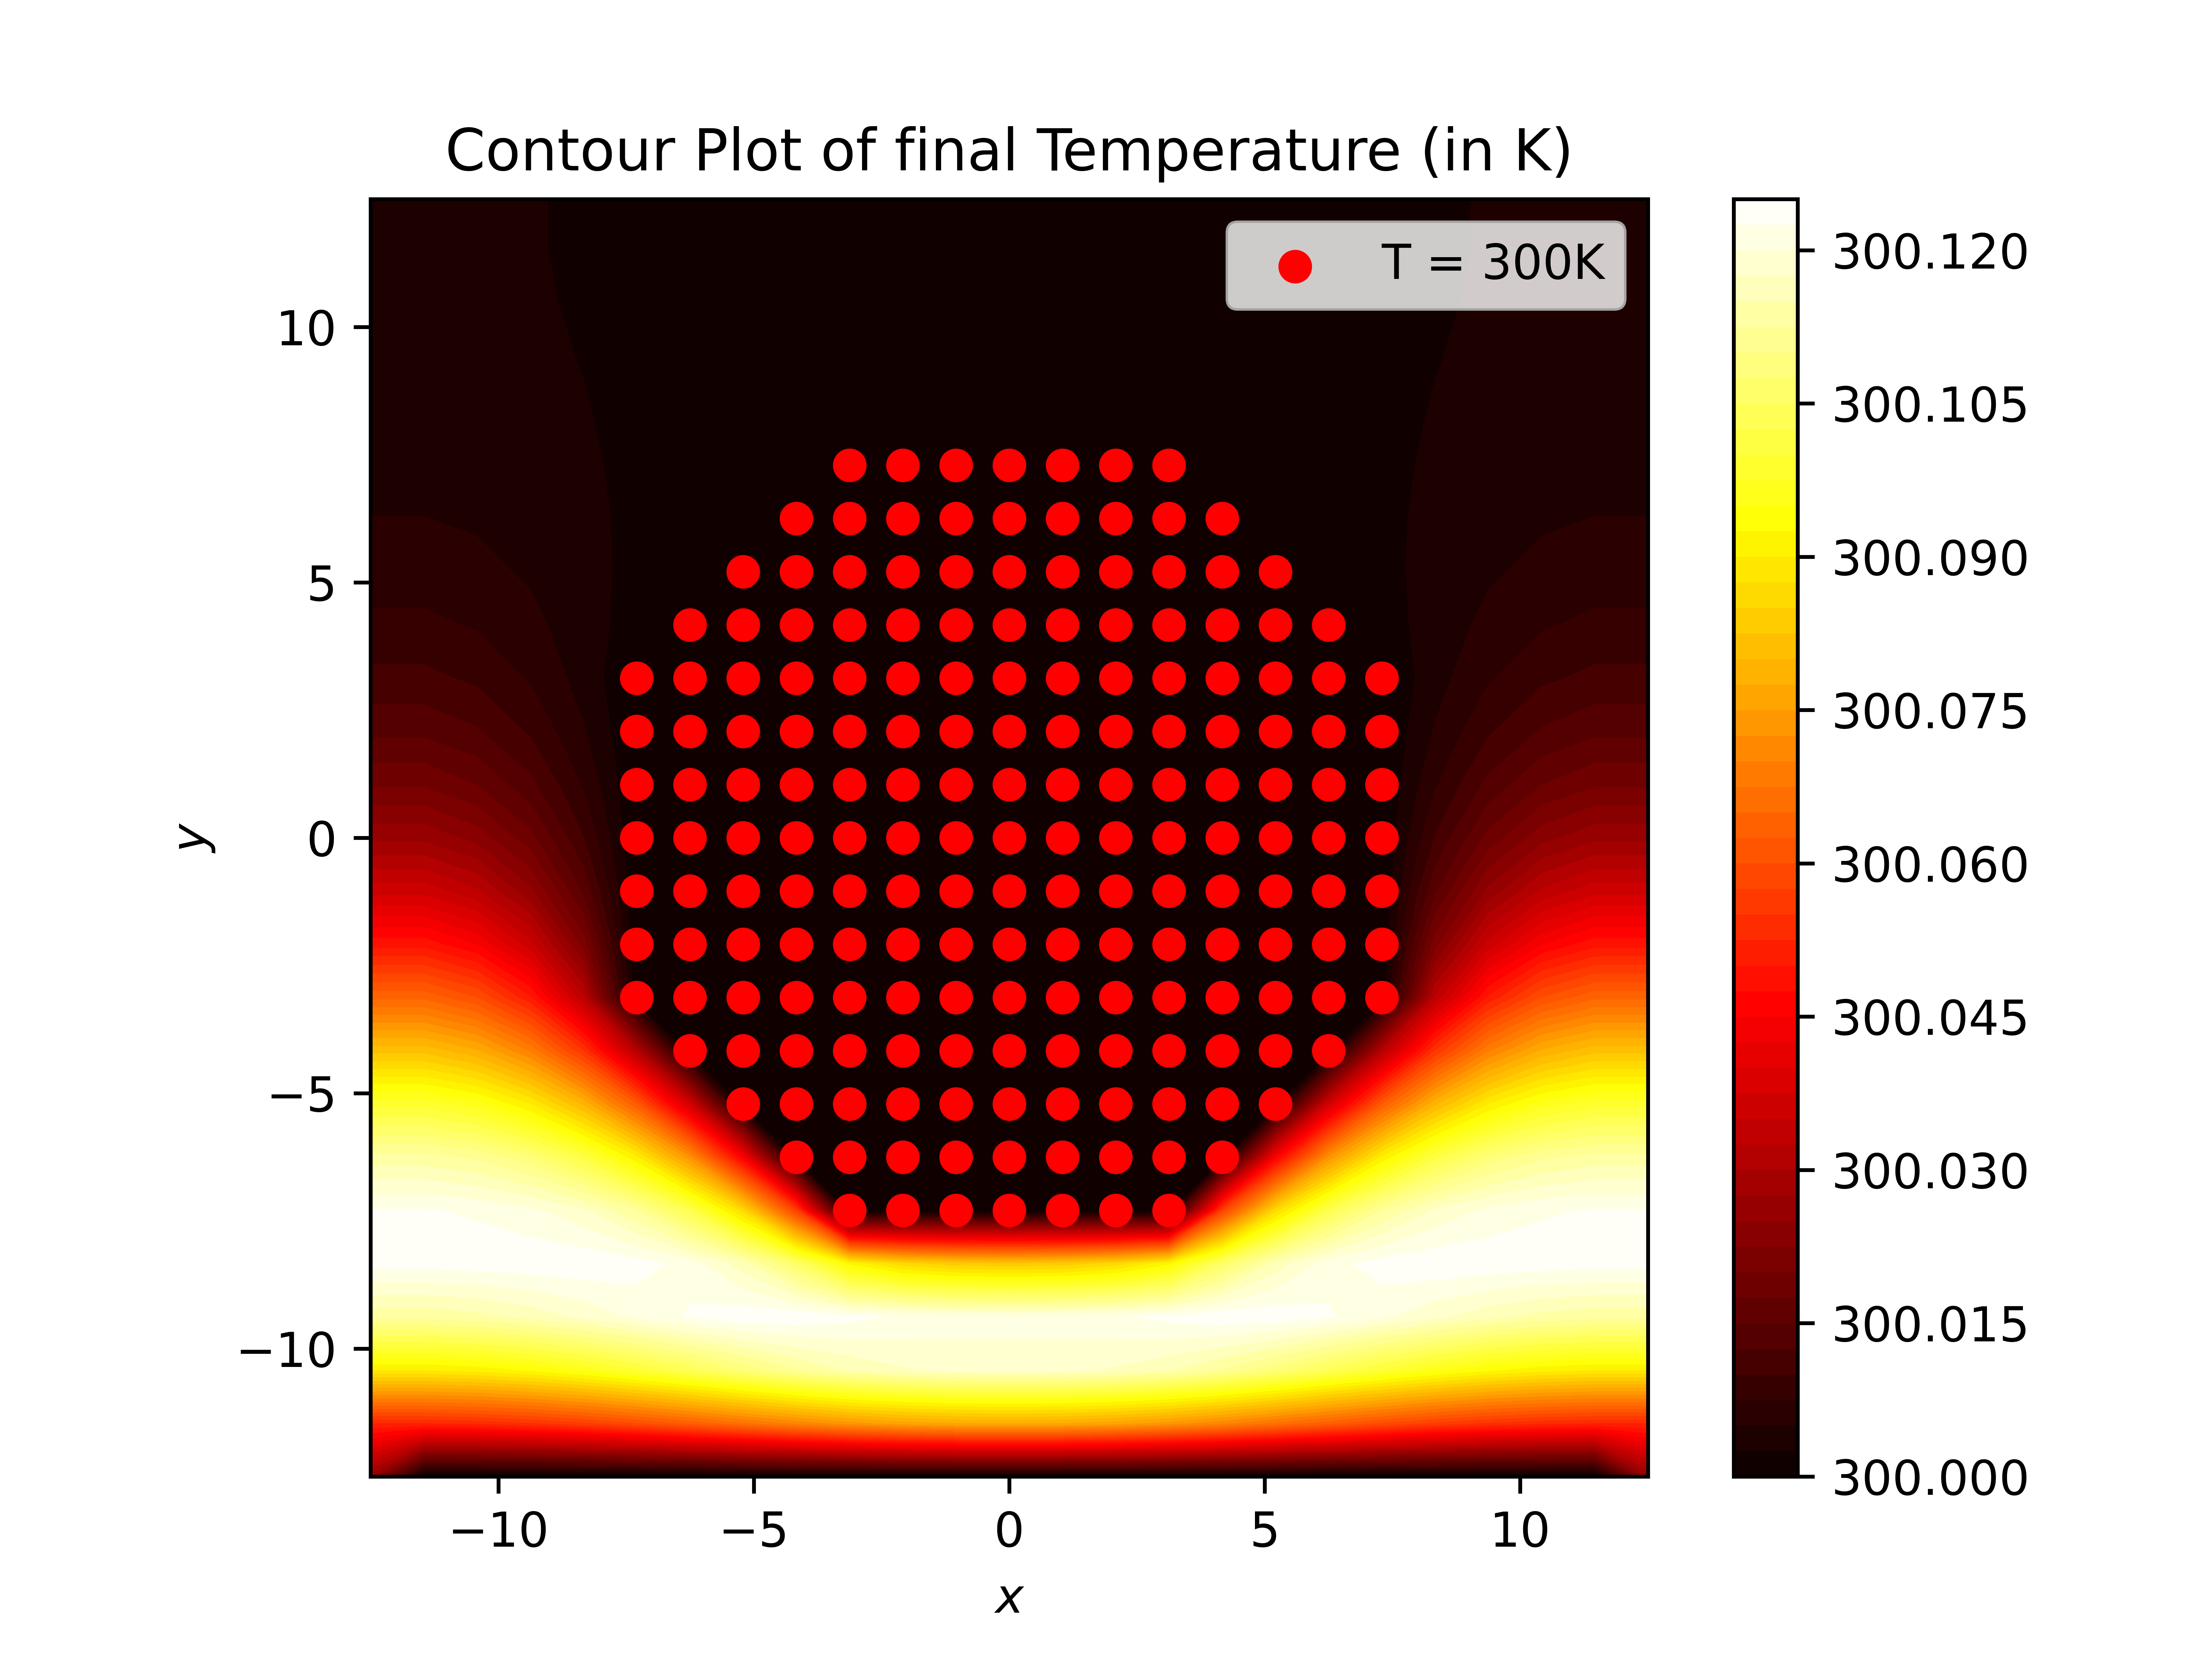
\includegraphics{images/fig7.png}
\end{center}

Note that the temperature differences are extremely exaggerated since the maximum temperature difference is only 0.12K.

Also, the regions where the current is flowing most are the hottest, as can be seen in this graph with the quiver plot superimposed over the contour plot:

\begin{center}
    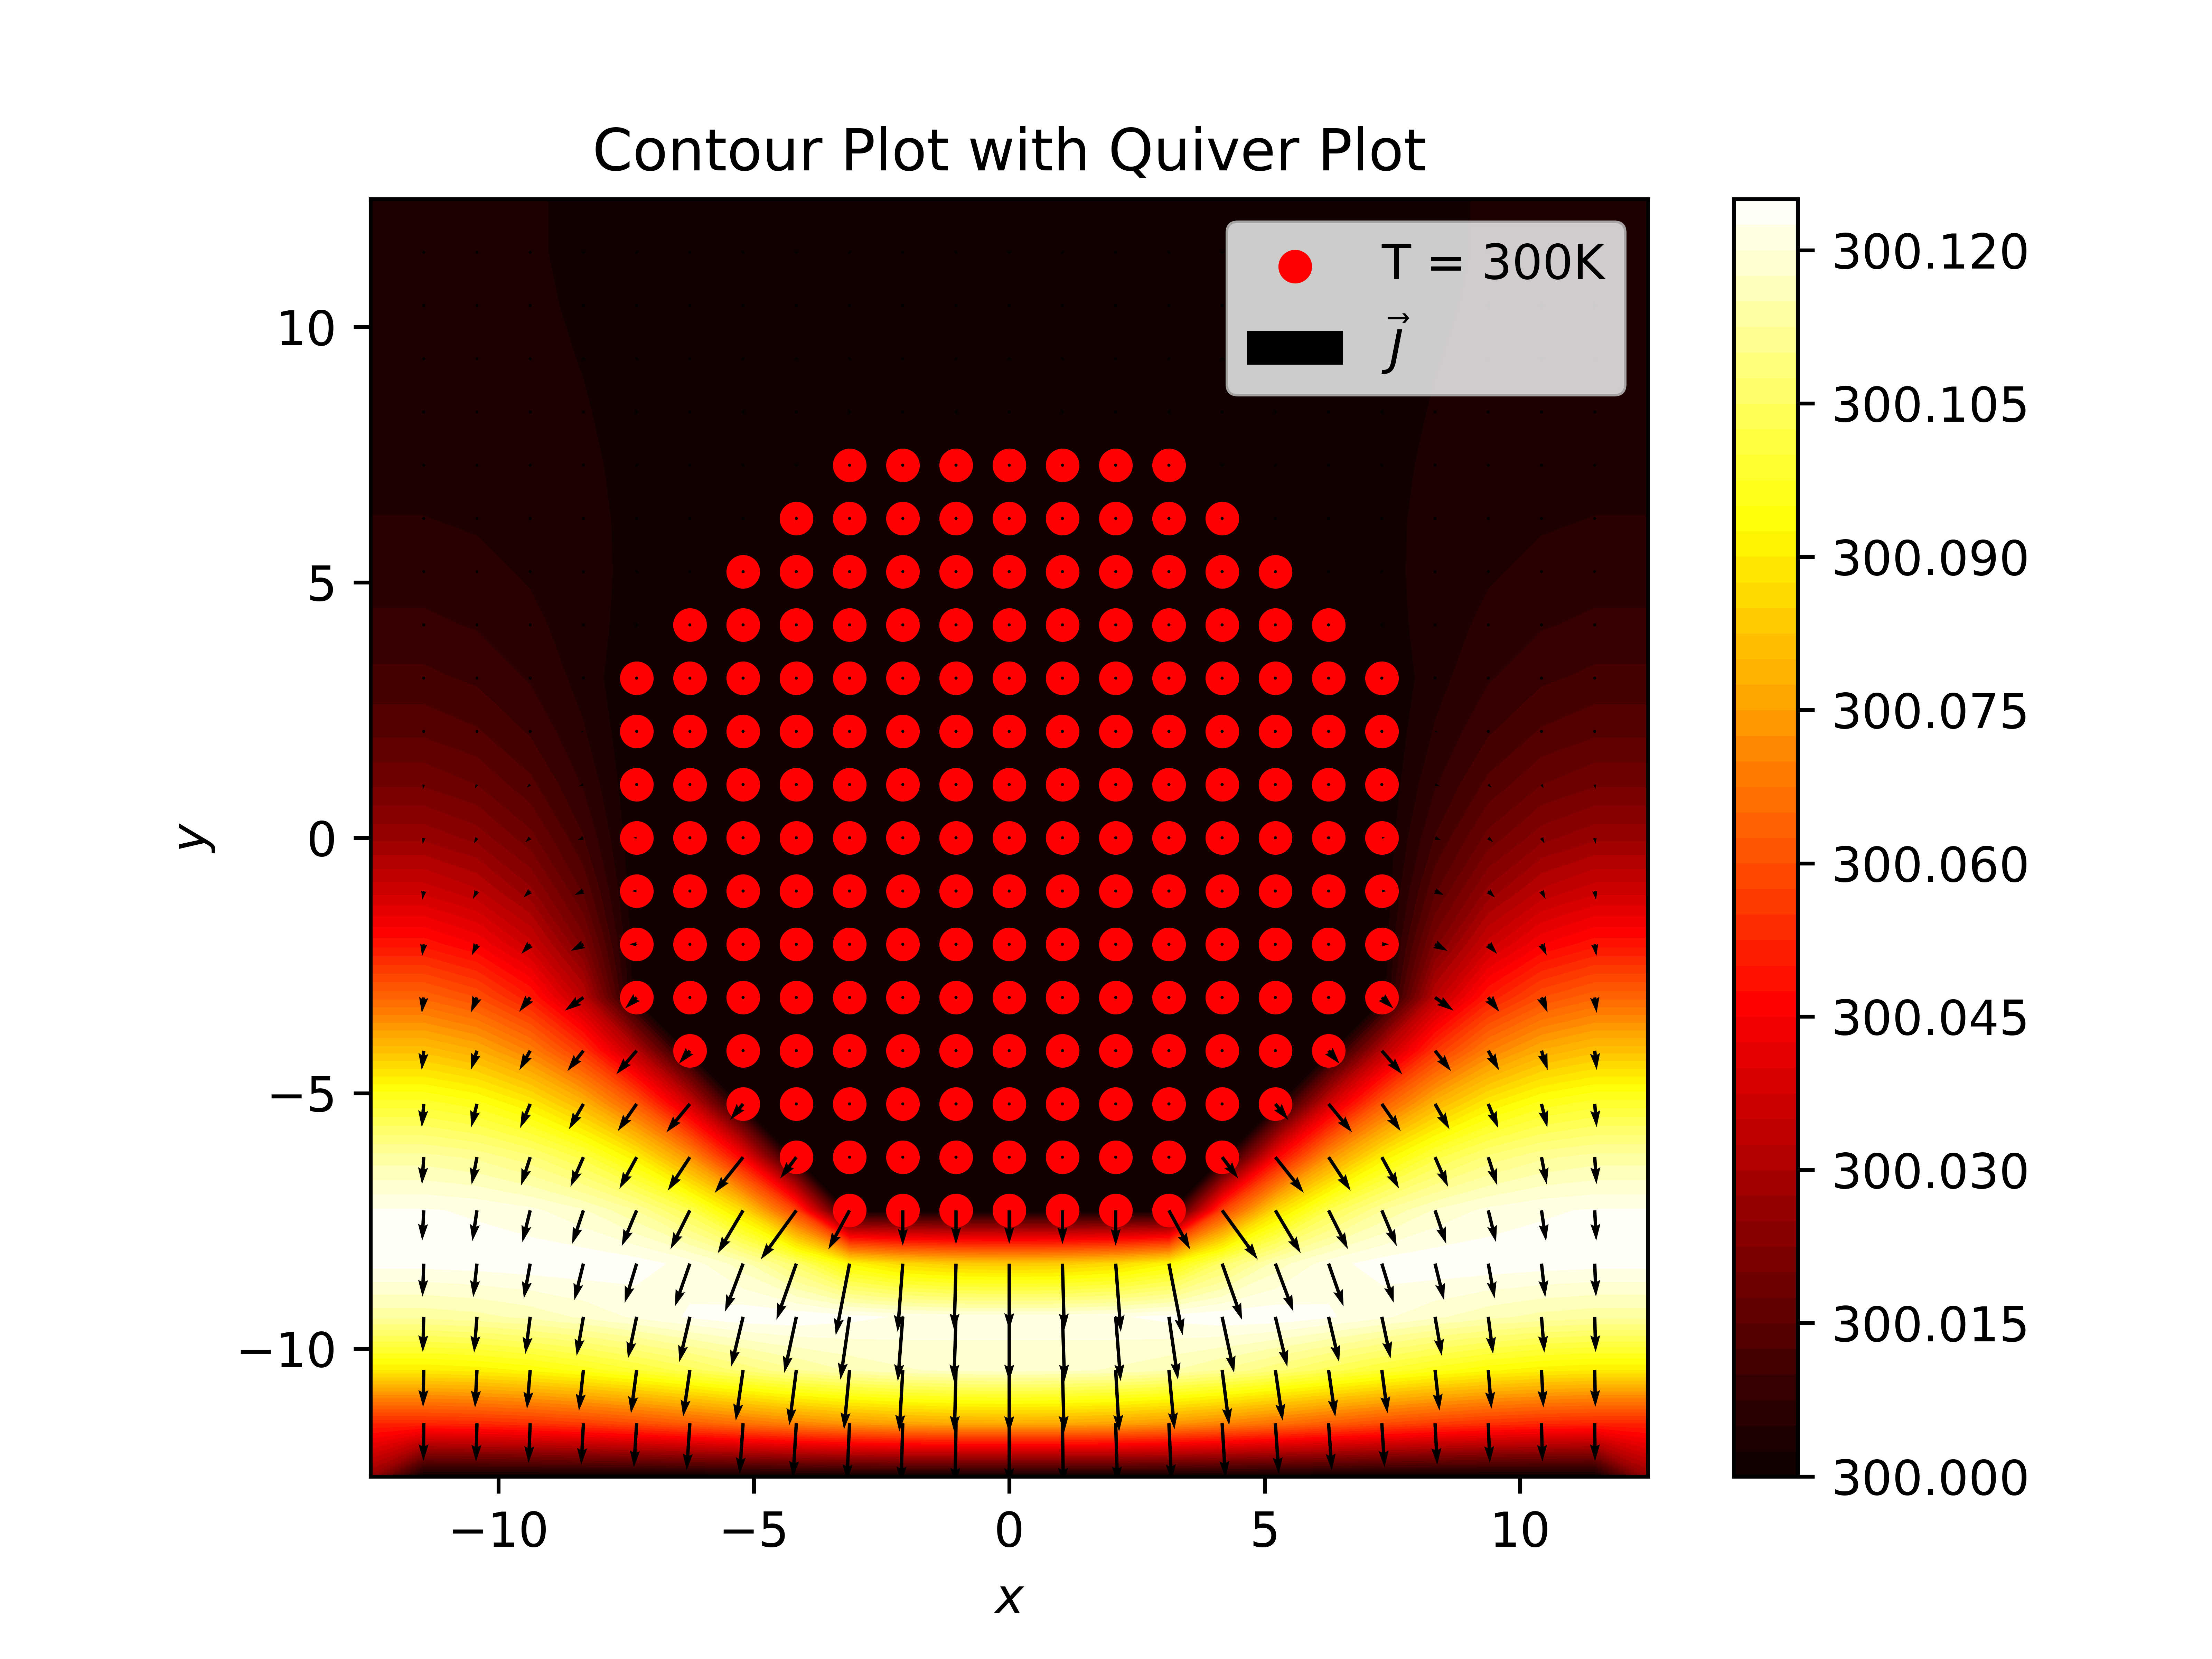
\includegraphics{images/fig8.png}
\end{center}
\pagebreak
\section{Conclusions}
\subsection{Conclusions regarding the Potential and Temperature Distributions}
\begin{itemize}
    \item The Potential Distribution results in a gradient that causes current to flow from the electrode contact to the grounded edge
    \item Most of the current hence flows from the center to the bottom edge
    \item As a result, the temperature of the region with the most current is the highest
\end{itemize}

\subsection{General Conclusions}
\begin{itemize}
    \item Solving the Laplace Equation in this manner is not very efficient, but it gives accurate results
\end{itemize}

\end{document}
